\chapter{Results}\label{chap:res_and_lit}

\section{Testing for termination}

\paragraph{}
The tests ran over all the (counter) satisfiable \ac{epr} problems in TPTP v6.1.0, and they were 267 problem. Only 101, which represents 37.8\%, were terminated within 3 minutes time limit and 1GB memory limit. Table ~\ref{table:sat_epr_results} shows detailed results of running all the 267 problem with the time needed to terminate the problem.
Another test were made but this time with 5 min. time limit and 2GB memory limit, and the results showed more 2 problems to terminate within that limit. Table ~\ref{table:more_sat_epr_results} shows the details of those 2 problems.
\paragraph{}
Figure ~\ref{fig:res_dist} is a pie chart that shows the distribution of the terminated 101 problems with respect of rating of the problem. 


\begin{figure}[H]
\centering
\begin{tikzpicture}
[
    pie chart,
    slice type={comet}{blu},
    slice type={legno}{rosso},
    slice type={coltello}{giallo},
    slice type={sedia}{viola},
    slice type={caffe}{verde},
    pie values/.style={font={\small}},
    scale=3
]

%81.65/0.00 Rating,
%      16.51/0.17 Rating,
%      1.83/0.33 Rating
    \pie[values of coltello/.style={pos=1.1}]%
        {}{81.19/comet,18.81/coltello}
   
    \legend[shift={(-1.5cm,-1cm)}]{{0.00 Rating}/comet}
    %\legend[shift={(0cm,-1cm)}]{{0.17 Rating}/sedia}
    \legend[shift={(1.5cm,-1cm)}]{{0.17 Rating}/coltello}

\end{tikzpicture}
\caption{Distribution of terminated problems over different ratings\label{fig:res_dist}}
\end{figure}

\paragraph{}
Table \ref{table:category_solved} shows how many problems were terminated in each category.
\begin{table}[H]
	\centering
	\begin{tabular}{|| c | c | c ||}
		\toprule
		Category & Number of problems & Number of problems terminated \\
		\midrule
		GRP & 50 & 15 \\
		HWV & 24 & 0 \\
		MGT & 2 & 0 \\
		NLP & 22 & 22 \\
		PUZ & 13 & 9 \\
		SYN & 114 & 32 \\
		HWC & 1 & 1 \\
		KRS & 24 & 19 \\
		MSC & 1 & 0 \\
		PLA & 4 & 0 \\
		SWB & 3 & 3 \\
		SYO & 9 & 0 \\
		\midrule
		Sum & 276 & 101 \\ 
		\bottomrule
	\end{tabular}
	\caption{Problems solved per category}
	\label{table:category_solved}
\end{table}

\paragraph{}
Some random problems were chosen to be tested thoroughly. SYN867-1 was one of them that gave interesting and weird results. The normal problem specification given to the prover terminated in 0.046s, however, when the transformed set was given to the prover, it did not terminate till 1000 seconds passed. So this shows that transformations may add a burden over the prover itself, since the transformations add a lot of new clauses to original problem specification. In the case of SYN867-1 problem, the original specification composed of 58 clauses, however it increased tremendously after the transformations to be 722.



\section{Testing for Model}\label{sec:test_model}
\paragraph{}
11 problems were chosen to test their explicit model; one time with applying the transformations, another time without applying them. The models in the 2 cases were exactly the same, the only difference was that the models with the transformations included extra elements for the domain predict introduced in the transformations. Also it is notable that the all 11 problems were almost range restricted from the beginning.

\paragraph{}
Those problems with their rating are listed in the below table:

\begin{table}[H]
	\centering
	\begin{tabular}{|| c | c || c | c ||}
		\toprule
		Problem & Rating & Problem & Rating \\
		\midrule
		PUZ001-3.p      &  0.00  &  PUZ080+2.p      &  0.00 \\		
		PUZ028-1.p      &  0.00  &  PUZ028-2.p      &  0.00 \\
		PUZ028-3.p      &  0.00  &  PUZ028-4.p      &  0.00 \\
		PUZ068+2.p      &  0.00  &  PUZ069+2.p      &  0.00 \\
		GRP125-4.004.p  &  0.17  &  GRP128-4.004.p  &  0.17 \\		
		GRP123-8.004.p  &  0.17  &                  &       \\
		\bottomrule
	\end{tabular}
	\caption{Problems used to test the Model}
	\label{table:mode_with_&_without}
\end{table}





%%%%%%%%%%%COMMENTS%%%%%%%%%%%%

\begin{comment}
\def\angle{0}
\def\radius{3}
\def\cyclelist{{"orange","blue","red","green"}}
\newcount\cyclecount \cyclecount=-1
\newcount\ind \ind=-1


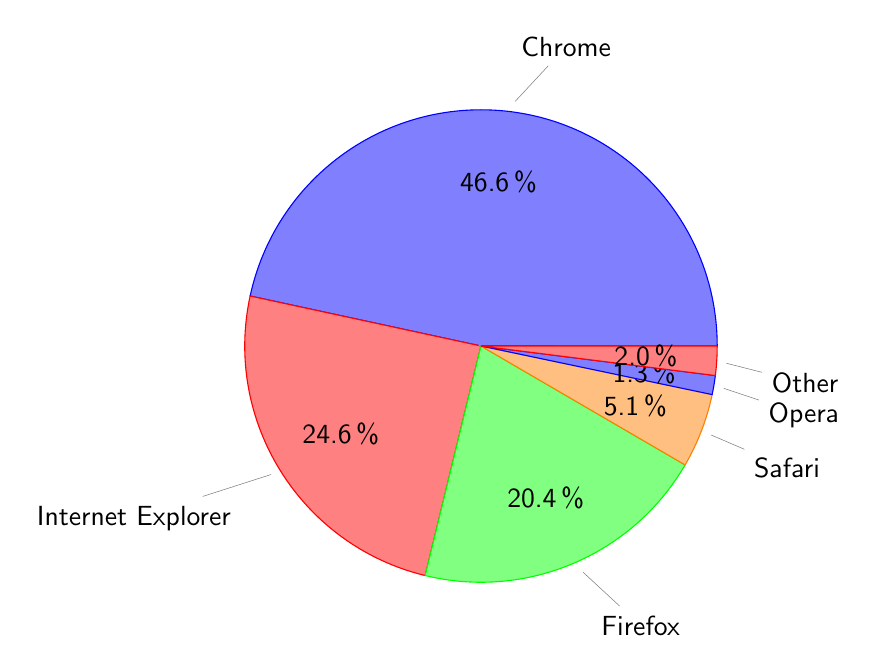
\begin{tikzpicture}[nodes = {font=\sffamily}]
  \foreach \percent/\name in {
      46.6/Chrome,
      24.6/Internet Explorer,
      20.4/Firefox,
      5.1/Safari,
      1.3/Opera,
      2.0/Other
    } {
      \ifx\percent\empty\else               % If \percent is empty, do nothing
        \global\advance\cyclecount by 1     % Advance cyclecount
        \global\advance\ind by 1            % Advance list index
        \ifnum3<\cyclecount                 % If cyclecount is larger than list
          \global\cyclecount=0              %   reset cyclecount and
          \global\ind=0                     %   reset list index
        \fi
        \pgfmathparse{\cyclelist[\the\ind]} % Get color from cycle list
        \edef\color{\pgfmathresult}         %   and store as \color
        % Draw angle and set labels
        \draw[fill={\color!50},draw={\color}] (0,0) -- (\angle:\radius)
          arc (\angle:\angle+\percent*3.6:\radius) -- cycle;
        \node at (\angle+0.5*\percent*3.6:0.7*\radius) {\percent\,\%};
        \node[pin=\angle+0.5*\percent*3.6:\name]
          at (\angle+0.5*\percent*3.6:\radius) {};
        \pgfmathparse{\angle+\percent*3.6}  % Advance angle
        \xdef\angle{\pgfmathresult}         %   and store in \angle
      \fi
    };
\end{tikzpicture}




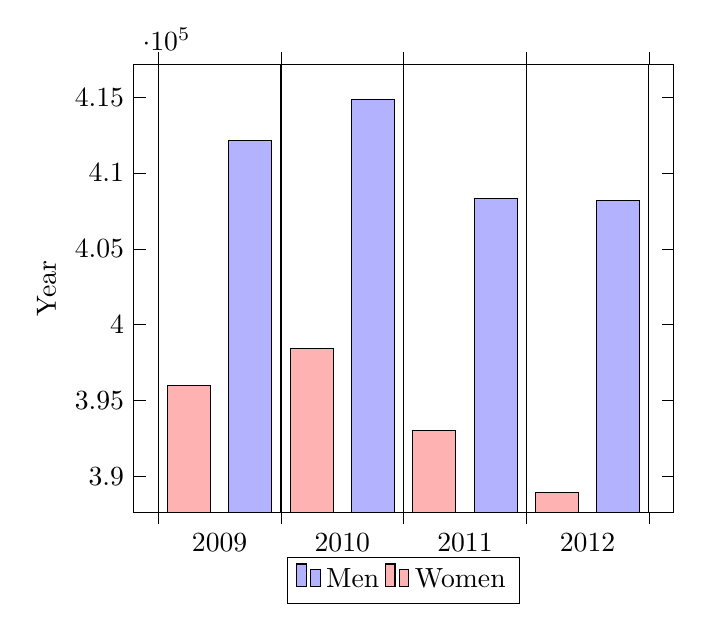
\begin{tikzpicture}
\begin{axis}[
	x tick label style={
		/pgf/number format/1000 sep=},
	ylabel=Year,
	enlargelimits=0.05,
	legend style={at={(0.5,-0.1)},
	anchor=north,legend columns=-1},
	ybar interval=0.7,
]
\addplot 
	coordinates {(2012,408184) (2011,408348)
		 (2010,414870) (2009,412156) (2008,415 838)};
\addplot 
	coordinates {(2012,388950) (2011,393007) 
		(2010,398449) (2009,395972) (2008,398866)};
\legend{Men,Women}
\end{axis}
\end{tikzpicture}



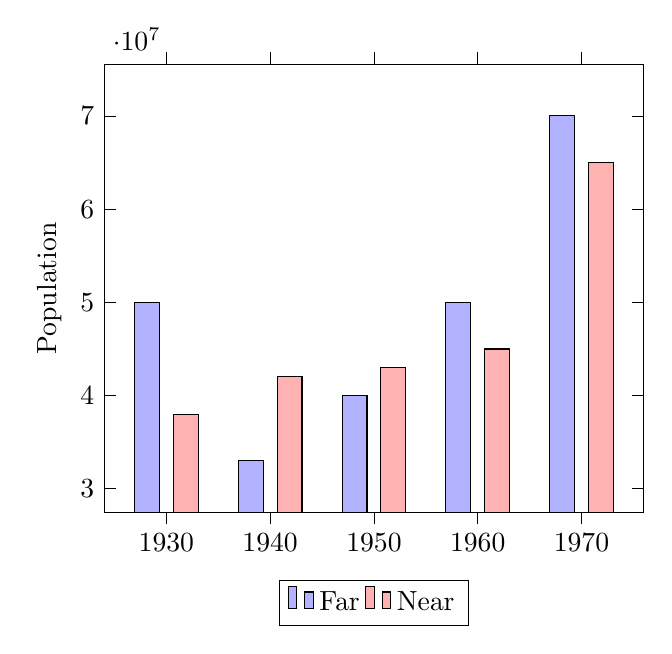
\begin{tikzpicture}
\begin{axis}[
	x tick label style={
		/pgf/number format/1000 sep=},
	ylabel=Population,
	enlargelimits=0.15,
	legend style={at={(0.5,-0.15)},
		anchor=north,legend columns=-1},
	ybar=5pt,% configures `bar shift'
	bar width=9pt
]
\addplot 
	coordinates {(1930,50e6) (1940,33e6)
		 (1950,40e6) (1960,50e6) (1970,70e6)};

\addplot 
	coordinates {(1930,38e6) (1940,42e6) 
		(1950,43e6) (1960,45e6) (1970,65e6)};

\legend{Far,Near}
\end{axis}
\end{tikzpicture}
\end{comment}